\chapter{テスト章}

この章はテスト用の章です。数式、図、表の例を示します\cite{example}。

\section{数式の例}

数式を以下に示します:

\begin{equation}
    \label{eq:test}
    E = mc^2
\end{equation}

式\eqref{eq:test}はアインシュタインの質量エネルギー等価性を表します。

\section{図の例}

図の例を以下に示します:

\begin{figure}[H]
    \centering
    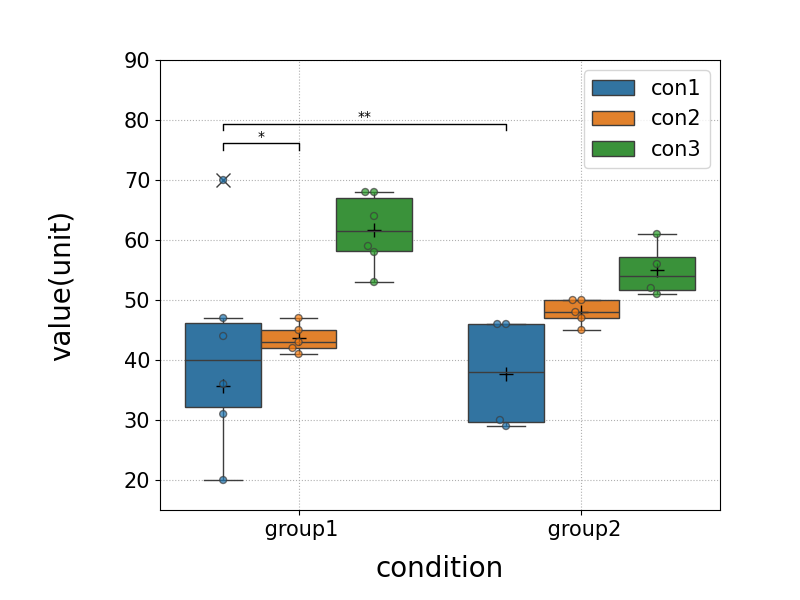
\includegraphics[width=0.8\textwidth]{figures/test/test.png} % サイズを指定
    \caption{テスト図}
    \label{fig:test}
\end{figure}

図\ref{fig:test}はテスト用の図です。

\section{表の例}

表の例を以下に示します:

\begin{table}[H]
    \centering
    \caption{テスト表}
    \label{tab:test}
    \begin{tabular}{|c|c|}
        \hline
        項目 & 値 \\
        \hline
        a & b \\
        c & d \\
        \hline
    \end{tabular}
\end{table}

表\ref{tab:test}はテスト用の表です。
